%%
%% 2019 07 04 Ph. G. Freimann
%%

\section{Zahlen}
\sectuntertitel{Im 15. Jahrhundert --- genauer im Jahre 1413 --- am
  zwölften elften um zehn Uhr neun haben acht der sieben Schlauesten
  gesagt: ``So sechs wie wir fünf gibt's keine vier mehr, denn wir
  drei sind die zwei einzigen Nullen.``}

Einführende Youtube Videos: \texttt{youtu.be/9JgcETAN65c} und \texttt{youtu.be/tPfnEByx9r0}

\theorieTALS{8}{1.1}
\theorieGESO{13}{1.1}
%%%%%%%%%%%%%%%%%%%%%%%%%%%%%%%%%%%%%%%%%%%%%%%%%%%%%%%%%%%%%%%%%%%%%%%%%%%%%%%%%
\subsection*{Lernziele}

\begin{itemize}
	\item Zahlmengen $\mathbb{N}$, $\mathbb{Z}$, $\mathbb{Q}$, $\mathbb{R}$
  \item Näherungswerte, Signifikante Ziffern, Runden
  \item Wissenschaftliche Notation
  \item Ordnungsrelationen ($=$, $<$, $>$, $\leq$, $\geq$)
  \item Betrag
\end{itemize}

\subsection{Die natürlichen Zahlen ($\mathbb{N}$)}\index{Zahlen!natürliche}

\begin{definition}{natürliche Zahlen}{definition_natuerliche_zahlen}
  Natürliche Zahlen $\mathbb{N}$ sind ganze positive Zahlen: ${1, 2, 3, 4, 5, ....}$.
\end{definition}

\begin{bemerkung}{}{}
  Selten wird auch die Menge ${0, 1, 2, 3, 4, ...}$ als die Menge
  der natürlichen Zahlen bezeichnet. Wir bezeichnen diese Menge dann mit $\mathbb{N}_0$.

  \TALS{%%
  Wenn Verwechslungen relevant würden, verwenden wir manchmal
  \begin{itemize}  
\item $\mathbb{N}^{\ast}$ oder $\mathbb{N}\backslash\{0\}$ für die Zahlen $\{1, 2, 3, 4, 5, ...\}$
  und
\item $\mathbb{N}_0$ für die Zahlen $\{0, 1, 2, 3, 4, ...\}$.
  \end{itemize}}%% END TALS

\end{bemerkung}
\newpage


\subsection{Ganze Zahlen ($\mathbb{Z}$)}
\begin{definition}{ganze Zahlen}{definition_ganze_zahlen}

  Mit $\mathbb{Z}$ bezeichnen wir alle ganzen Zahlen, sowohl die
  positiven ($\mathbb{N}$), wie auch die negativen.
  \end{definition}

$$\mathbb{Z} = \{..., -3, -2, -1, 0, 1, 2, 3,  4, ... \}$$

\subsubsection{Zahlenstrahl / Zahlengerade}\index{Zahlenstrahl}

\begin{center}
\raisebox{-1cm}{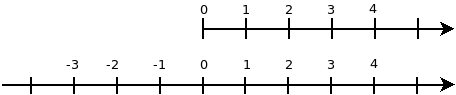
\includegraphics[width=13cm]{allg/alg/img/Zahlenstrahl.png}}
\end{center}

Der Zahlenstrahl hat den Startpunkt 0 (Null)\footnote{... manchmal  den Startpunkt 1 ...}, wohingegen die
Zahlengerade auf beiden Seiten uneingeschränkt weiterläuft.

\subsection{Rationale Zahlen ($\mathbb{Q}$)}
\index{Zahlen!rationale}\index{rationale Zahlen}

\begin{definition}{rationale Zahlen}{}
Zahlen, welche sich als Bruch mit ganzen Zahlen schreiben lassen,
werden als \textbf{rationale Zahlen} bezeichnet.


$$\mathbb{Q} =\left\{ q = \frac{a}{b} \,\,\, \middle| \,\,\, a \in \mathbb{Z}, b \in \mathbb{N}\right\}$$
\end{definition}

\subsubsection{Dezimalbrüche}\index{Dezimalbruch}
Jeder Bruch bestehend aus ganzen Zahlen ($\frac{a}{b}$) lässt sich als
abbrechender oder periodischer Dezimalbruch schreiben. Beispiel:

$$\frac{5}{70} = 0.0\overline{714285}$$

Dasselbe gilt umgekehrt. Für abbrechende Dezimalbrüche ist dies
trivial:
$$47.386 = \frac{47\,386}{1\,000}$$

Für periodische, nicht abbrechende Dezimalbrüche sieht die Sache etwas komplizierter aus,
gilt jedoch auch:

$$0.\overline{13} = 0.131313... = 13: 99 = \frac{13}{99}$$

\TRAINER{Bem.: $\frac{1}{9} = 0.111\overline{1}$, $\frac{1}{99} = 0.0101\overline{01}$, $\frac{1}{999} = 0.001001\overline{001}$, ...}

%%\GESOAadB{22}{7. a) b) c) d) e)}
\newpage


\subsection{Runden}\index{runden}
In der Regel sind wir bei Dezimalbrüchen nicht an allen auftretenden
Stellen interessiert, sondern begnügen uns mit einer Näherung.

\subsubsection{Dezimale (Nachkommastelle)}\index{Dezimale}\index{Nachkommastelle}
Als Dezimale, Dezimalstelle oder Nachkommastelle werden die Stellen \textbf{nach} dem Komma bezeichnet.
Runden auf die vierte \textbf{Dezimale} (= vierte \textbf{Nachkommastelle}):
$$ 36.4699432 \approx  \LoesungsRaum{36.4699}$$
$$ 36.4699618 \approx  \LoesungsRaum{36.4700}$$
\textbf{Vorsicht} bei Zahlen nahe an Null. So wird die Zahl
$$0.002468$$ beim Runden auf vier Dezimalen wie folgt gerundet:
$$0.0025$$

Runden Sie auf {\color{ForestGreen}vier} Dezimalen:

\begin{tabular}{rcl}
  $55.55555$      &$\approx$& \LoesungsRaum{$55.{\color{ForestGreen}\mathbf{5556}}$}\\
  $8.55695$       &$\approx$& \LoesungsRaum{$8.{\color{ForestGreen}\mathbf{5570}}$}\\
  $3.3339499$     &$\approx$& \LoesungsRaum{$3.{\color{ForestGreen}\mathbf{3339}}$}\\
  $1000.0001$     &$\approx$& \LoesungsRaum{$1000.{\color{ForestGreen}\mathbf{0001}}$}\\
  $10\,000.00001$ &$\approx$& \LoesungsRaum{$10\,000.{\color{ForestGreen}\mathbf{0000}}$}\\
  $-6.99999$      &$\approx$& \LoesungsRaum{$-7.{\color{ForestGreen}\mathbf{0000}}$}\\
  $0.000040447$   &$\approx$& \LoesungsRaum{$0.{\color{ForestGreen}\mathbf{0000}}$}\\
\end{tabular}

\TRAINER{Das letzte Beispiel zeigt, dass so oft wichtige Information
  verloren geht. Daher wird sinnvollerweise meist auf signifikante Stellen, und nicht
  auf Dezimalen gerundet.}
\newpage


\begin{rezept}{Auf signifikante Ziffern runden}{}
  
  Beim Runden auf \textbf{vier signifikante Ziffern} wird
  \begin{itemize}
  \item  von links nach rechts die erste von Null verschiedene Ziffer gesucht. Dies ist die
    erste signifikante Ziffer.
  \item
    Danach werden die nächsten drei Ziffern
  genommen, egal ob sie Null sind oder nicht. 
\item   Mit diesen drei Ziffern bilden die Ziffern zusammen die vier
  signifikanten Ziffern.
\item  Die 5. Ziffer wird nur noch zum Auf- oder Abrunden verwendet.
  \end{itemize}
\end{rezept}

Geben Sie {\color{ForestGreen}\textbf{vier}} \textbf{signifikante} Ziffern an und runden Sie wenn nötig:

$$0.000040447  \approx \LoesungsRaum{0.0000{\color{ForestGreen}\mathbf{4045}}}$$
$$36.4699432 \approx \LoesungsRaum{{\color{ForestGreen}\mathbf{36.47}}}$$
$$36.9952831 \approx \LoesungsRaum{{\color{ForestGreen}\mathbf{37.00}}}$$
$$30009.78   \approx \LoesungsRaum{{\color{ForestGreen}\mathbf{3001}}0}$$
$$0.0439899  \approx \LoesungsRaum{0.0{\color{ForestGreen}\mathbf{4399}}}$$
$$1\,000\,000 \approx \LoesungsRaum{{\color{ForestGreen}\mathbf{1\,000}}\,000}$$
$$0.00001    \approx \LoesungsRaum{0.0000{\color{ForestGreen}\mathbf{1000}}}$$
\newpage

  
\subsubsection{Wissenschaftliche Notation}\index{Notation!wissenschaftliche}\label{wissenschaftlicheNotation}
Bei Zahlen größer als 10 können wir einer Zahl manchmal nicht ansehen, wie viel Stellen denn nun signifikant sind.

$$ 679946 \textrm{\ Einwohner} \approx  680000 \textrm{\ Einwohner}$$
$$ 680023 \textrm{\ Einwohner} \approx  680000 \textrm{\ Einwohner}$$

Daher bietet sich die wissenschaftliche Notation an.\footnote{Die
\textbf{wissenschaftliche Notation} wird vorwiegend für sehr große
aber auch für Zahlen sehr nahe an Null verwendet.}
Bei der wissenschaftlichen Notation wird die erste signifikante Ziffer
vor das Komma geschrieben. Nach dem Komma stehen \textbf{alle} weiteren signifikanten Stellen.
Zuletzt wird die Zahl mit Zehnerpotenzen
($10^{n}: n \in \mathbb{Z}$) «an die richtige Stelle» gerückt:

$$64\,038.6  = 6.40386 \cdot 10^{ 4}\approx 6.40 \cdot 10^{ 4}$$
$$0.00463640 = 4.63640 \cdot 10^{-3}\approx 4.64 \cdot 10^{-3}$$

Dabei bezeichnen negative Exponenten die Zehntel, Hundertstel, etc.
Erst in der wissenschaftlichen Notation können wir die signifikanten Stellen auch bei gerundeten Zahlen größer als 10 effektiv ablesen.

\TALS{S. \cite{frommenwiler17alg} S. 40 Kap. 1.5.5}


\paragraph{Taschenrechner} Auf Taschenrechnern oder in
Programmiersprachen wird die Exponentialschreibweise i.\,d.\,R. mit dem
Buchstaben «e» angegeben. Also «e$n$» anstelle von «$\cdot10^{n}$». Beispiele:

$5\,000 = 5\, \cdot 10^{3} = 5\mathrm{e}3$

$0.063 = 6.3\, \cdot 10^{-2} = 6.3\mathrm{e-}2$

\GESO{%%
  \begin{rezept}{}{}
    Um 5.77 Millionen auf Ihrem Taschenrechner \textbf{einzugeben} tippen Sie:

\begin{center}  5.77 \tiprobutton{EE} 6 \end{center}

    \end{rezept}
  }%% END GESO
\newpage

\subsection{Irrationale und reelle Zahlen ($\mathbb{R}$)}\index{Zahlen!reelle}

  Zahlen auf der Zahlengerade, welche nicht als Bruch $\frac{a}{b}$ mit $a\in\mathbb{Z}$, $b \in \mathbb{N}$ dargestellt werden können, werden als \textbf{irrational}\index{irrational} bezeichnet.

Wichtigste Vertreter:

\begin{center}
\raisebox{-3.9cm}{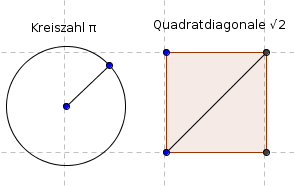
\includegraphics[width=6.5cm]{allg/alg/img/IrrationaleZahlen.png}}
\index{Pi, Kreiszahl}\index{$\sqrt{2}$ Wurzel aus zwei}\index{$\pi$ (Kreiszahl)}
\end{center}

\begin{definition}{Reelle Zahl}{}
Die Vereinigungsmenge der rationalen ($\mathbb{Q}$) und der irrationalen Zahlen
nennen wir die \textbf{reellen} Zahlen und bezeichnen die Menge mit $\mathbb{R}$.
\end{definition}

\begin{gesetz}{Zahlmengen Beziehungen}{}
$$\mathbb{N} \subset \mathbb{Z} \subset \mathbb{Q} \subset \mathbb{R} $$
\end{gesetz}

\bbwCenterGraphic{8cm}{allg/alg/img/nzqr.png}

Dass $\pi$ oder $\sqrt{2}$ irrational sind, ist nicht trivial. Daher
noch zwei Vertreter irrationaler Zahlen, bei denen sofort klar ist,
dass es sich nicht um periodische Dezimalbrüche handelt:
\begin{itemize}
\item $0.10 100 100010000100000100000010000000...$
\item $0.12345678910111213141516 ... 9899100101102103104 ... $
\end{itemize}
\newpage


\subsection*{Aufgaben zum Kapitel Zahlmengen}
\GESOAadB{22ff}{5., 6.}
\TALSAadB{13}{14-18}

%%\TRAINER{
%%\subsection{Mengenlehre}
%%\begin{itemize}
%%\item Venn-Diagramme
%%\item Mengenoperationen
%%\item Zahlmengen
%%\end{itemize}
%%}
